%%%%%%%%%%%%%%%%%%%%%%%%%%%%%%%%%%%%%%%%%
% fphw Assignment
% LaTeX Template
% Version 1.0 (27/04/2019)
%
% This template originates from:
% https://www.LaTeXTemplates.com
%
% Authors:
% Class by Felipe Portales-Oliva (f.portales.oliva@gmail.com) with template 
% content and modifications by Vel (vel@LaTeXTemplates.com)
%
% Template (this file) License:
% CC BY-NC-SA 3.0 (http://creativecommons.org/licenses/by-nc-sa/3.0/)
%
%%%%%%%%%%%%%%%%%%%%%%%%%%%%%%%%%%%%%%%%%

%----------------------------------------------------------------------------------------
%	PACKAGES AND OTHER DOCUMENT CONFIGURATIONS
%----------------------------------------------------------------------------------------

\documentclass[
	12pt, % Default font size, values between 10pt-12pt are allowed
	%letterpaper, % Uncomment for US letter paper size
	%spanish, % Uncomment for Spanish
]{../Template/fphw}

% Template-specific packages
\usepackage[utf8]{inputenc} % Required for inputting international characters
\usepackage[T1]{fontenc} % Output font encoding for international characters
\usepackage{mathpazo} % Use the Palatino font

\usepackage{graphicx} % Required for including images

\usepackage{booktabs} % Required for better horizontal rules in tables

\usepackage{listings} % Required for insertion of code

\usepackage{enumerate} % To modify the enumerate environment

% Additional packages needed
\usepackage{amsmath}
\usepackage{enumitem}
\usepackage{mwe}
\usepackage{comment}
\usepackage{listings}
\usepackage{xcolor}
\usepackage{tikz}

\lstset{
  language=Python,
  basicstyle=\ttfamily\small,
  keywordstyle=\color{blue},
  stringstyle=\color{red},
  commentstyle=\color{green},
  morecomment=[l][\color{magenta}]{\#},
  frame=single, % adds a frame around the code
  breaklines=true, % sets automatic line breaking
  breakatwhitespace=true, % sets if automatic breaks should only happen at whitespace
  tabsize=4, % sets default tabsize to 4 spaces
  showstringspaces=false % Instructs Listings to not put marks in string spaces
}

%----------------------------------------------------------------------------------------
%	ASSIGNMENT INFORMATION
%----------------------------------------------------------------------------------------

\title{Homework \#3} % Assignment title

\author{Mao Nishino} % Student name

\date{March 28th, 2024} % Due date

\institute{Florida State University \\ Department of Computer Science} % Institute or school name

\class{Deep and Reinforcement Learning Fundamentals (CAP5619-0001.sp24)} % Course or class name

\professor{Dr. Xiuwen Liu} % Professor or teacher in charge of the assignment

%----------------------------------------------------------------------------------------

\begin{document}

\maketitle % Output the assignment title, created automatically using the information in the custom commands above

%----------------------------------------------------------------------------------------
%	ASSIGNMENT CONTENT
%----------------------------------------------------------------------------------------

\section*{Question 1}

\begin{problem}
 Convolutional neural networks are very successful in practical applications, especially in object
classification. Explain the following common components in CNNs and how they contribute to their successes.
\begin{enumerate}[label=(\arabic*)]
\item (4 points) Convolutional layers (including their sparse connectivity and parameter sharing).
\item (2 points) Pooling layers.
\item (3 points) Learned kernels (i.e., the weights after a CNN is trained).
\item (3 points) The depth of convolutional layers (see Figure 9.4 in the textbook for some hints).
\item (3 points) The fully connected layers.
\end{enumerate}
\end{problem}

%------------------------------------------------

\subsection*{Answer}
Let us denote the set of 3D arrays of shape $(A,B,C)$ by $\mathbb{R}^{A\times B\times C}$. Define the notation for 4D arrays similarly.
\begin{enumerate}[label=(\arabic*)]
    \item A (2D) \textbf{convolutional} layer takes a 2D image $I \in \mathbb{R}^{C\times H\times W}$ ($C$ is the number of channels such as R, G, and B channels for RGB images, $H$ is the height of the image, $W$ is the width of the image) and outputs another image $J \in \mathbb{R}^{C_{out}\times H_{out}\times W_{out}}$ defined by
    \begin{equation}
        J_{ijk} = \sum_{l=1}^{C}\sum_{m,n=1}^{r} I_{l,m+sj, n+sk}K_{i,l,m,n}
    \end{equation}
    where $K\in \mathbb{R}^{C_{out}\times C\times r\times r}$ is an array of learnable weights called the \textbf{kernel}, $r$ is called the kernel size, $C_{out}$ is the number of output features (a hyperparameter), $s$ is the step size of the kernel called the \textbf{stride} and  $H_{out},W_{out}$ are the shape of the output image (determined from $H,W,r,s$ so that $1\leq m+sj\leq H, 1\leq n+sk\leq W$ i.e. the kernel does not go out of the image).
    The three main ideas of a convolutional layer are \textbf{sparse connections}, \textbf{parameter sharing}, and \textbf{equivariance to translation}. Unlike fully connected layers, each pixel in the output image is NOT connected to all pixels in the previous layer. Instead, it is connected to only a small part of the image defined by the kernel size. This allows for the efficient detection of local features such as edges. Indeed, to find an edge, we do not have to look at the whole image; we only have to look at a small part of it. This idea is called \textbf{sparse connections}. Now, if we look at the formula above, we notice that the kernel is shared at all locations in the image. In other words, the \textbf{parameters} are \textbf{shared} at all locations. This idea allows us to drastically reduce the number of parameters to learn and allows more flexibility. For example, the above formula is well-defined even if the images are of variable shape. If we use fully connected layers, we can only accept images of fixed shapes because the number of parameters is tied to the image shape. Finally, since the parameters are shared, if we translate the input image, the output image shows the same features, just translated by the same degree. This is called an \textbf{equivariance to translation}. Because of this, we can detect the same features at different locations in the same way. This is useful for geometric features like edges since we frequently observe similar edges in one image.

    \item After applying a convolutional layer, it is common to apply an activation function (such as ReLU). After applying an activation, the result goes through a \textbf{pooling layer}. A pooling layer is a type of layer rather than one specific architecture, and two common layers that belong to this category are a \textbf{max pooling} layer and a \textbf{average pooling} layer. As a max pooling layer is much more common, we focus on it for explanation. A max pooling layer takes an image $I\in (C,H,W)$ and outputs $J\in (C,H_{out},W_{out})$ where
    \begin{equation}
        J_{i,j,k} = \max_{m,n= 1,\cdots r} I_{i, m+sj, n+sk}
    \end{equation}
    where $s,r,H_{out},W_{out}$ are defined in the same way as a convolutional layer. The main motivation for the pooling layer is to gain \text{invariance to small translation}. Consider a 1D array [1,5,3,2,5]. If we apply max pooling to this array with kernel size 3 and stride 1, we obtain [5,5,5], and this does not change even if we translate the array left or right (assuming the values coming outside of the array are $0$). Therefore, after applying max pooling, the output does not change for small translations. This is useful, especially for images, because we often don't need exact pixel information on features. In the above example, channels do not interact with each other, but if we take a maximum across the channels, a max pooling layer can be invariant to other transformations. For example, if we have three channels, each detects an edge in three directions, a max pooling layer would output a high value as long as at least one of the three directions is detected, meaning a max pooling layer can act like an "OR" gate, so we can detect all three directions of the edges. Pooling layers also help with dimension reduction because a pooling operation reduces the size of images drastically. By reducing the size, we can improve the computational efficiency. It also has a regularizing effect since we will have fewer parameters, restricting the model's capability to overfit.

    \item We already discussed some ideas on a kernel $K$ in (1), so let us review some and add to it. One of the most important ideas for a kernel was that, unlike fully connected layers, the kernel (weights) are shared. This allows us to reduce computational expense while gaining equivariance to translation. Moreover, by having many channels in the output (i.e., having a large $C_{out}$), the kernel can learn many different features, such as edges in different directions. By using this together with max pooling in (2), we can make our models invariant to some geometric transformations, and this can help in making the model robust.
    
    \item By increasing the depth of convolutional layers, we can learn more complex and larger features of the image. Although each convolutional layer only looks at a very small part of the image, by stacking convolutional layers, layers in the later part of the network can indirectly see a large part of the image because each pixel in the output of a convolutional layer is a summary of multiple pixels in the input, so repeatedly summarizing the pixels would give us a summary of many pixels in the original image.

    \item Fully connected layers in convolutional neural networks come after applying stacks of convolutional layers and pooling as the last layers. They are responsible for describing nonlinear interactions between all features detected in convolutional layers. Since all neurons interact with each other, these layers can have a global view of the image, which is something the convolutional layers cannot do since they are localized by definition. More practically, if we would like to solve classification tasks, the output of the network should be a vector of probabilities where the size is equal to the number of classes. On the other hand, the convolutional layers output a 3-dimensional tensor, which does not quite match what we need. Fully connected layers can reduce the dimension and match the dimension to what we need.
\end{enumerate}
 
%----------------------------------------------------------------------------------------

\section*{Question 2}

\begin{problem}
In the deep learning framework you have established, train a convolutional neural network or
obtain a pretrained model on the MNIST dataset. You can use any program and model available to you as long as there
are at least three convolutional layers and the accuracy on the training set is at least 95\%. Answer the following
questions:
\begin{enumerate}[label = (\arabic*)]
\item (8 points) Visualize the filters (as images) in the first three convolution layers. Then explain the patterns you
observe.
\item (4 points) Visualize the feature map of the third convolutional layer (i.e., the output from the third convolutional
layer) for a digit ‘0’ and a digit ‘8’ (which are classified correctly). By comparing the two feature maps, could
you tell the important discriminant features between the two digits (i.e., the features that can be used to
distinguish them)?
\item  (8 points) Shift a digit ‘7’ (which is classified correctly initially) to the left five pixels, and to the right five
pixels, will the prediction by the network change? Then classify them using the convolutional neural network
you have trained or obtained. Here fill the missing values using the closest valid ones (i.e., using the clamp
border padding method). You can choose any image for digit '7' that is classified correctly.
\end{enumerate}
\end{problem}

%------------------------------------------------

\subsection*{Answer}

\begin{enumerate}[label = (\arabic*)]
    \item Figure \ref{fig:filters} shows the filters in each layer. In the first layer, Filter 1 shows one very negative point with positive values surrounding it.   As we will see in Figure \ref{fig:feature_maps_0}, this layer seems to detect the background of the image. On the other hand, in Filter 2, we see a bright vertical line at the center, which could be a detector for bright spots in the image, which is confirmed by Figure \ref{fig:feature_maps_0}. In the second layer, the common theme is that we have at least one black dot surrounded by brighter dots. In particular, we observe the U-shaped filter in 1 and 2, while we observe a gradient of the intensity in 3 and the reverse L shape in 4. Finally, in Layer 3, we observe more complex shapes. In Filter 1, we observe a T shape with a dot added, and this seems to be in charge of detecting a horizontal line in Figure \ref{fig:feature_maps_0}. On the other hand, we see a diagonal line in Filter 2 from the middle left to the bottom center, which detects the diagonal in the same direction. In Filter 3, we see a clear H shape that detects diagonal lines from right to left, and in Filter 4, we see a gradient from the top left to the bottom right.
    \begin{figure}[!htbp]
        \centering 
        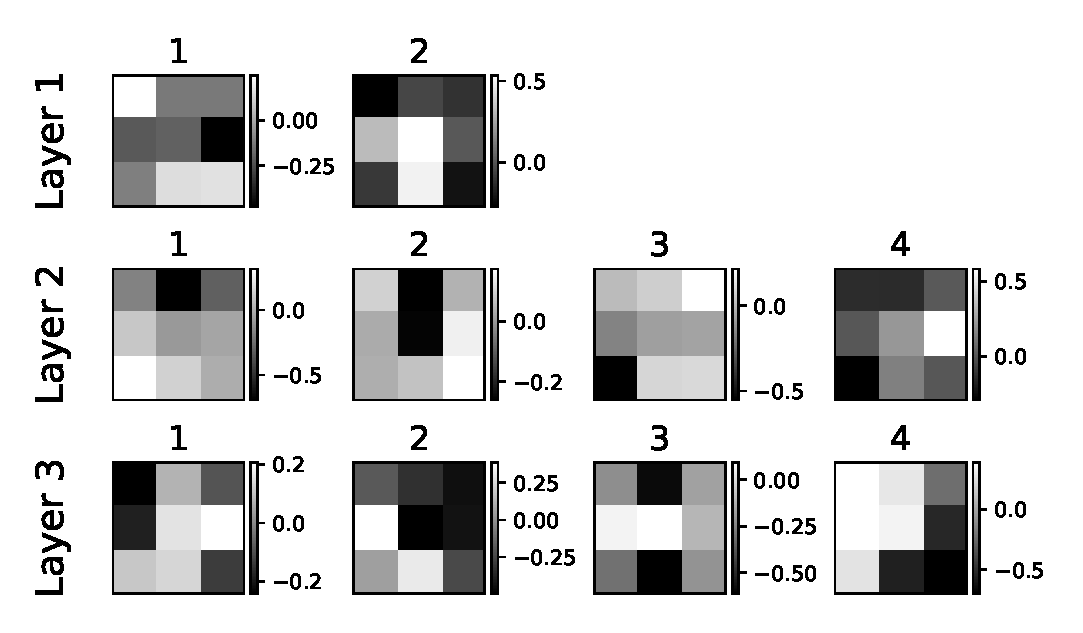
\includegraphics{codes/filters}
        \caption{Filters in each layer. }
        \label{fig:filters}
    \end{figure}
    \item Figure \ref{fig:feature_maps_0} and \ref{fig:feature_maps_8} show the feature maps at all three convolutional layers, and the feature maps we are asked for are shown at the bottom. We note that features 2 and 3 in the last layers show their biggest differences. As we have seen earlier, these features seem to detect diagonal lines, and the number of diagonal lines is distinctively different in those two digits. Therefore, features 2 and 3 can be used to distinguish 0 and 8.
    \begin{figure}[!htbp]
    \centering
    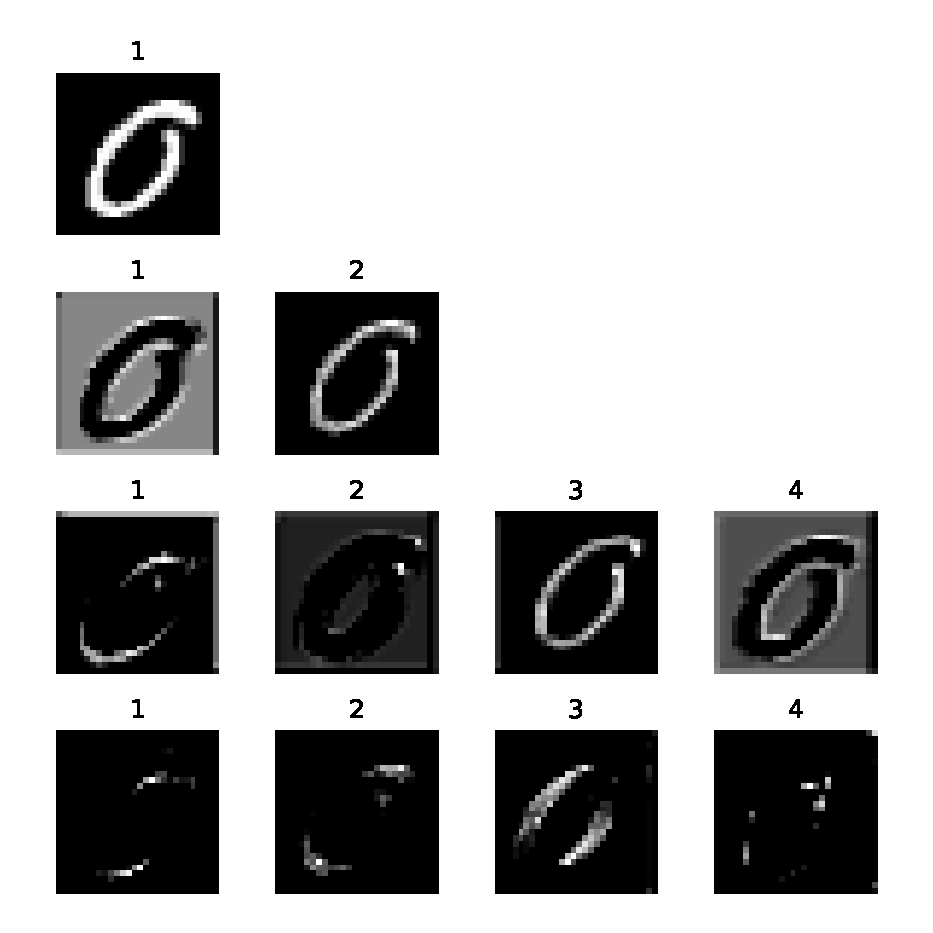
\includegraphics{codes/feature_maps_0}
    \caption{The feature maps for a digit $0$. The first column shows the original image (the input layer), and the following rows show the feature maps at each layer in ascending order.}
    \label{fig:feature_maps_0}
    \end{figure}

    \begin{figure}[!htbp]
    \centering
    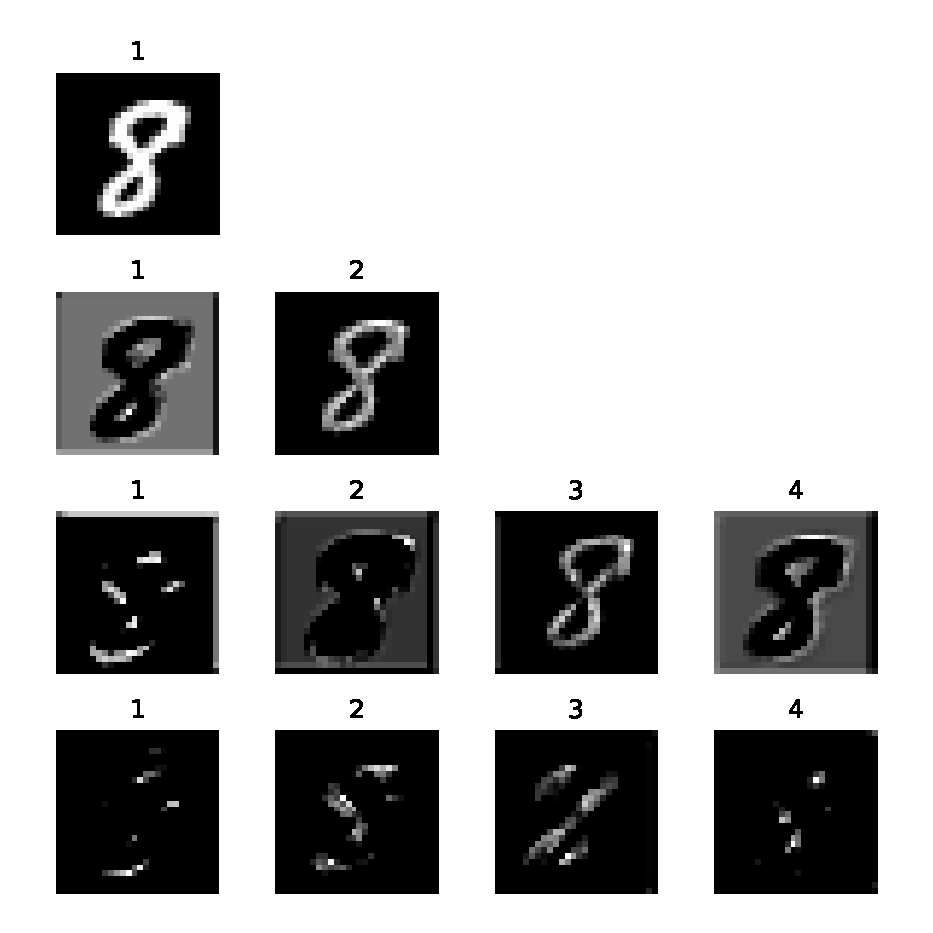
\includegraphics{codes/feature_maps_8}
    \caption{The feature maps for a digit $8$. The first column shows the original image (the input layer), and the following rows show the feature maps at each layer in ascending order}
    \label{fig:feature_maps_8}
    \end{figure}

    \item Figure \ref{fig:translated_7} shows the original image and translated images. Our experiment showed that all of these images are correctly classified as $7$, showing the robustness to the translation.
    \begin{figure}[!htbp]
        \centering
        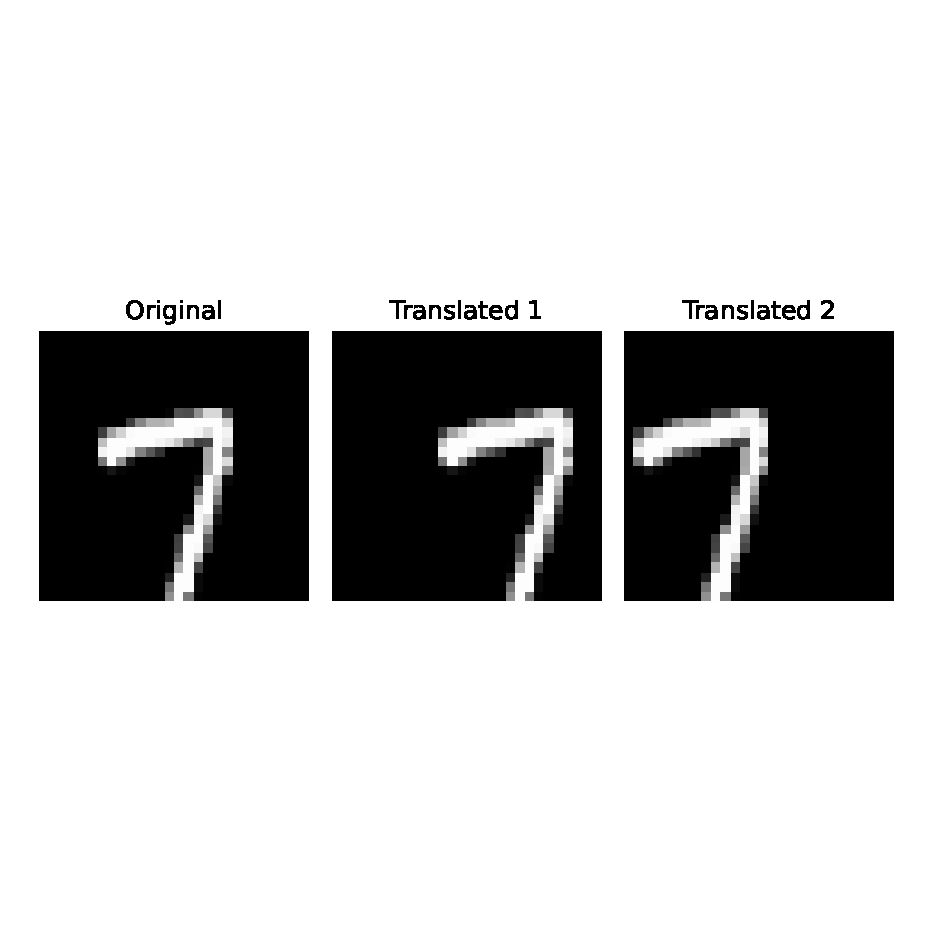
\includegraphics[width=\textwidth]{codes/translated_images}
        \caption{The original digit seven and translated images. }
        \label{fig:translated_7}
    \end{figure}
\end{enumerate}

%----------------------------------------------------------------------------------------

\section*{Question 3}

\begin{problem}
Here we empirically test the robustness of the model you have for Problem 3. Imagine that we
have a 8x8 black patch and we move it from left to right, from top to down with a stride of 1 to occlude part of the
image. Using a digit ‘6’ (which is classified correctly initially) as an example, answer the following questions.
\begin{enumerate}[label=(\arabic*)]
\item (12 points) Create three maps (i.e., images) in the following way. For each valid position of the black patch
(i.e., every pixel in the black patch covers a valid original pixel), store the probability of ‘6’ of the partially
covered image in map 1, the highest probability (among the 10 classes) in map 2, and classified label (‘0’ to
‘9’) in map 3. Display the maps. Make sure that they are clearly legible by scaling values.
\item (4 points) By analyzing the maps, explain which parts of the ‘6’ are important for recognition.
\item (4 points) Based on your result, would you be able to create “adversarial” images(i.e., to be classified as another
digit) by covering some parts of ‘6’ using patches from the images of the other digits? (See “The Elephant in
the Room,” available from https://arxiv.org/pdf/1808.03305.pdf for examples on other datasets). 
\end{enumerate}
\end{problem}

%------------------------------------------------

\subsection*{Answer} 
\begin{enumerate}[label=(\arabic*)]
    \item Figure \ref{fig:Q3_1} shows all the required maps along with the original image used to create the map.
    \begin{figure}[!htbp]
        \centering
        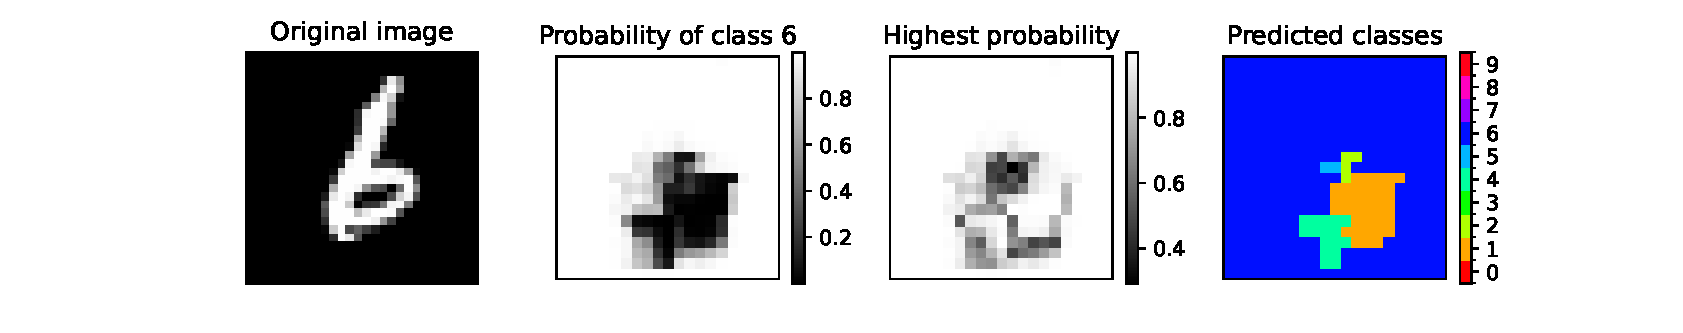
\includegraphics[width=\textwidth]{codes/P3_1}
        \caption{Maps required in (1). }
        \label{fig:Q3_1}
    \end{figure}
    \item We observe that the O-shaped part of the digit 6 seems to be the most important feature. If the O-shape's right side is obscured, it will be classified as 1, while if we obscure the bottom left part, it will be classified as 4, and this result aligns with our intuition.
    \item Figure \ref{fig:hw3adversarial} shows the original image and the adversarial image made by patching a part of digit 2 to the image. As we observe in the figure, the classification is altered by modifying the O-shaped in the digit.
    \begin{figure}[!htbp]
        \centering
        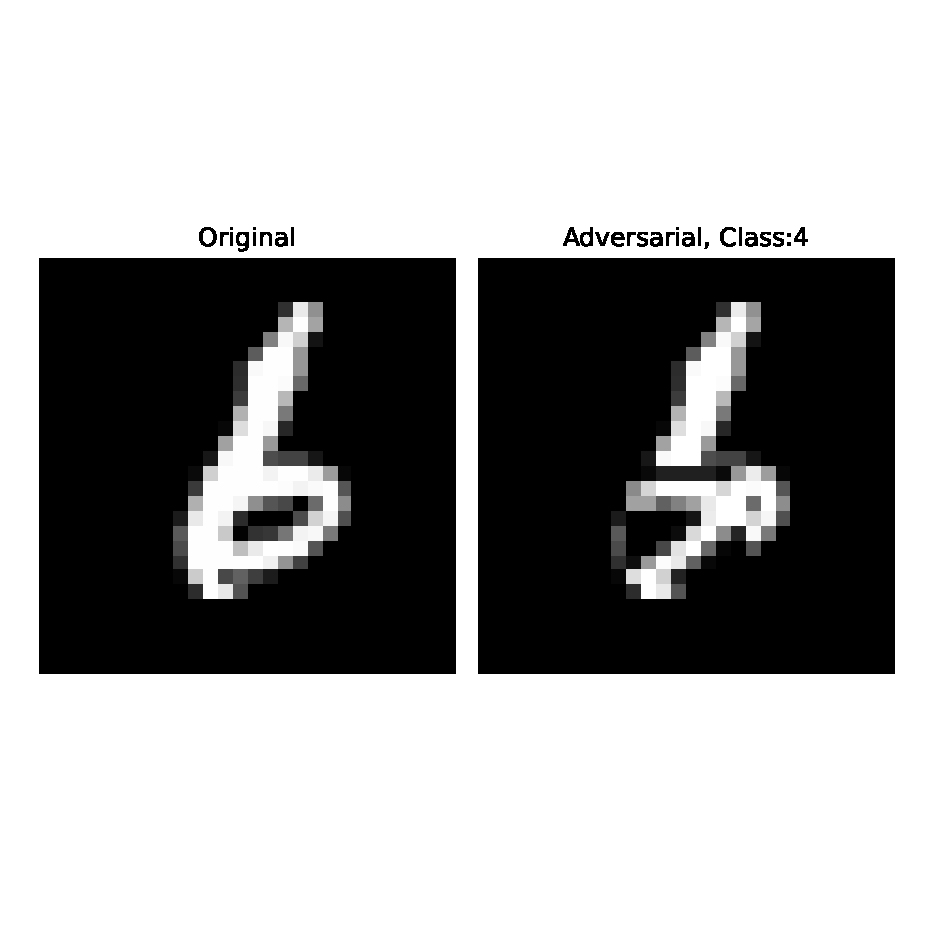
\includegraphics{codes/adversarial_image}
        \caption{The original image and a patched image. The part of the digit 2 was used to patch the image.}
        \label{fig:hw3adversarial}
    \end{figure}
\end{enumerate}

%----------------------------------------------------------------------------------------

\section*{Question 4}

\begin{problem}
The main purpose of this problem is to gain a deeper understanding of the back-propagation through time algorithm for a recurrent neural network via an example. We will use the recurrent neural network defined by equations (10.8) to (10.11) (in the Deep Learning textbook) with a customized loss function:
\[
L(x^{(1)}, \ldots, x^{(\tau}) = (\hat{y}^{(\tau)}_2 - 0.25)^2 - \log(\hat{y}_{1}^{(\tau)}).
\]
and the following parameter values:
\[
b = \begin{bmatrix} -1 \\ 1 \end{bmatrix}, \quad
c = \begin{bmatrix} 0.5 \\ -0.5 \end{bmatrix}, \quad
W = \begin{bmatrix} 1 & -1 \\ 0 & 2 \end{bmatrix}, \quad
U = \begin{bmatrix} -1 & 0 \\ 1 & -2 \end{bmatrix}, \quad
V = \begin{bmatrix} -2 & 1 \\ -1&0 \end{bmatrix},
\]
for the following sequence:
\[
x^{(1)} = \begin{bmatrix} 1 \\ 0 \end{bmatrix}, \quad
x^{(2)} = \begin{bmatrix} 0.5 \\ 0.25 \end{bmatrix}, \quad
x^{(3)} = \begin{bmatrix} 0 \\ 1 \end{bmatrix},
\]
where \(\tau=3\).
\begin{enumerate}[label=(\arabic*)]
    \item (8 points) Write a program that computes the outputs and loss using the given sequence and parameter values. Give \(\hat{y}^{(t)}\) (i.e., \(\hat{y}^{(t)}_1\) and \(\hat{y}^{(t)}_2\)) for \(t=1\) to 3 and the customized loss.
    \item (2 points) Estimate the gradient of the loss function with respect to \(b_1\) and \(b_2\) using the central difference method using \(\epsilon=0.000025\).
    \item (4 points) Compute the gradient of the loss function with respect to \(b_1\) and \(b_2\) by unfolding the network through time. You need to show the intermediate results.
    \item (4 points) Fixing the other parameters, perform one step of gradient descent optimization on \(b_1\) and \(b_2\) using a learning rate of 0.005.
    \item (2 points) Use your program to compute the loss using the new values for \(b\) (with other parameters as given) for the original sequence.
\end{enumerate}
\end{problem}

%------------------------------------------------

\subsection*{Answer}

\begin{enumerate}[label=(\arabic*)]
    \item  The following is the code I used to output $\hat{y}^{(t)}$ and the loss. The calculated loss was \\ \verb|0.09796771659419912| and the value for $y$ was as follows:
    \begin{itemize}
        \item $\hat{y}^{(1)}$ = \verb|[0.94921601 0.05078399]|
        \item $\hat{y}^{(2)}$ = \verb|[0.95221995 0.04778005]|
        \item $\hat{y}^{(3)}$ = \verb|[0.94001124 0.05998876]|
    \end{itemize}
    \begin{lstlisting}[language=Python]
import numpy as np
import scipy.special as sps

x = np.zeros((3,2))
x[0] = np.array([1.,0.])
x[1] = np.array([0.5,0.25])
x[2] = np.array([0.,1.])
b = np.array([-1.,1.])
c = np.array([0.5,-0.5])
W = np.array([[1.,-1.],[0.,2.]])
U = np.array([[-1.,0.],[1.,-2.]])
V = np.array([[-2.,1.],[-1.,0.]])

def forward_prop(x, W, U, V, b, c, tau):
    h = np.zeros((tau,2))
    y = np.zeros((tau,2))
    for t in range(tau):
        if t == 0:
            h[t] = np.tanh(b + np.dot(U,x[t]))
        else:
            h[t] = np.tanh(b + np.dot(W,h[t-1]) + np.dot(U,x[t]))
        y[t] = sps.softmax(np.dot(V,h[t]) + c)
    loss = (y[tau-1][1] - 0.25)**2 - np.log(y[tau-1][0])
    return loss, y

loss, y = forward_prop(x, W, U, V, b, c, 3)
print(loss)
print(y[0], y[1], y[2])
    \end{lstlisting}
    \item The following shows the code to calculate the gradient via central difference. The estimated gradient with respect to $b$ was \verb|[ 0.00038813 -0.01691036]|.
    \begin{lstlisting}[language=Python]
# Estimate the gradient wrt b using central differences
eps = 0.000025
grad_b = np.zeros(2)
for i in range(2):
    b[i] += eps
    loss_plus, y = forward_prop(x, W, U, V, b, c, 3)
    b[i] -= 2*eps
    loss_minus, y = forward_prop(x, W, U, V, b, c, 3)
    grad_b[i] = (loss_plus - loss_minus)/(2*eps)
    b[i] += eps
print(grad_b)
    \end{lstlisting}
    \item Figure \ref{fig:comp_graph_rnn} shows our network's abbreviated computational graph and the unfolded graph leading up to the loss function. We will use this graph to compute the gradient.
    \begin{figure}[!htbp]
        \centering
\tikzset{every picture/.style={line width=0.75pt}} %set default line width to 0.75pt        

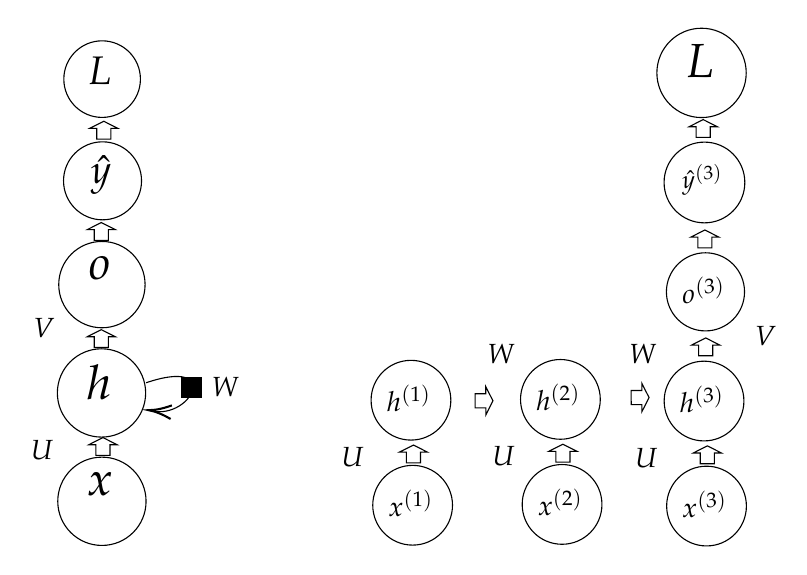
\begin{tikzpicture}[x=0.75pt,y=0.75pt,yscale=-1,xscale=1]
%uncomment if require: \path (0,300); %set diagram left start at 0, and has height of 300

%Up Arrow [id:dp5523402133850748] 
\draw   (178.8,115.84) -- (185.6,112.4) -- (192.4,115.84) -- (189,115.84) -- (189,121) -- (182.2,121) -- (182.2,115.84) -- cycle ;
%Up Arrow [id:dp12981233827516725] 
\draw   (178.8,167.44) -- (185.6,164) -- (192.4,167.44) -- (189,167.44) -- (189,172.6) -- (182.2,172.6) -- (182.2,167.44) -- cycle ;
%Up Arrow [id:dp8075948753634521] 
\draw   (179.6,219.44) -- (186.4,216) -- (193.2,219.44) -- (189.8,219.44) -- (189.8,224.6) -- (183,224.6) -- (183,219.44) -- cycle ;
%Curve Lines [id:da3620522985596637] 
\draw    (207.2,189.6) .. controls (243.67,177.18) and (229.34,206.92) .. (210.19,203.24) ;
\draw [shift={(208.4,202.8)}, rotate = 5.12] [color={rgb, 255:red, 0; green, 0; blue, 0 }  ][line width=0.75]    (10.93,-3.29) .. controls (6.95,-1.4) and (3.31,-0.3) .. (0,0) .. controls (3.31,0.3) and (6.95,1.4) .. (10.93,3.29)   ;
%Shape: Square [id:dp27455160672539725] 
\draw  [fill={rgb, 255:red, 0; green, 0; blue, 0 }  ,fill opacity=1 ] (224.4,187.2) -- (234,187.2) -- (234,196.8) -- (224.4,196.8) -- cycle ;
%Up Arrow [id:dp872448389408518] 
\draw   (329.2,223.04) -- (336,219.6) -- (342.8,223.04) -- (339.4,223.04) -- (339.4,228.2) -- (332.6,228.2) -- (332.6,223.04) -- cycle ;
%Up Arrow [id:dp7296375763069862] 
\draw   (401.2,222.64) -- (408,219.2) -- (414.8,222.64) -- (411.4,222.64) -- (411.4,227.8) -- (404.6,227.8) -- (404.6,222.64) -- cycle ;
%Up Arrow [id:dp49242579957404575] 
\draw   (469.6,119.44) -- (476.4,116) -- (483.2,119.44) -- (479.8,119.44) -- (479.8,124.6) -- (473,124.6) -- (473,119.44) -- cycle ;
%Up Arrow [id:dp1935940758536152] 
\draw   (470,171.44) -- (476.8,168) -- (483.6,171.44) -- (480.2,171.44) -- (480.2,176.6) -- (473.4,176.6) -- (473.4,171.44) -- cycle ;
%Up Arrow [id:dp03532246059737698] 
\draw   (470.8,223.44) -- (477.6,220) -- (484.4,223.44) -- (481,223.44) -- (481,228.6) -- (474.2,228.6) -- (474.2,223.44) -- cycle ;
%Up Arrow [id:dp027974251372299364] 
\draw   (370.84,191.5) -- (374.3,198.29) -- (370.88,205.1) -- (370.87,201.7) -- (365.71,201.71) -- (365.69,194.91) -- (370.85,194.9) -- cycle ;
%Up Arrow [id:dp463358826409326] 
\draw   (446.04,189.9) -- (449.5,196.69) -- (446.08,203.5) -- (446.07,200.1) -- (440.91,200.11) -- (440.89,193.31) -- (446.05,193.3) -- cycle ;
%Up Arrow [id:dp1720088488556819] 
\draw   (180,67.04) -- (186.8,63.6) -- (193.6,67.04) -- (190.2,67.04) -- (190.2,72.2) -- (183.4,72.2) -- (183.4,67.04) -- cycle ;
%Up Arrow [id:dp017957609940141506] 
\draw   (468.8,66.24) -- (475.6,62.8) -- (482.4,66.24) -- (479,66.24) -- (479,71.4) -- (472.2,71.4) -- (472.2,66.24) -- cycle ;

% Text Node
\draw    (185.9, 246.7) circle [x radius= 21.27, y radius= 21.27]   ;
\draw (177.4,231.6) node [anchor=north west][inner sep=0.75pt]  [font=\LARGE]  {$x$};
% Text Node
\draw    (185.7, 194.5) circle [x radius= 21.27, y radius= 21.27]   ;
\draw (177.2,179.4) node [anchor=north west][inner sep=0.75pt]  [font=\LARGE]  {$h$};
% Text Node
\draw    (185.9, 142.3) circle [x radius= 20.8, y radius= 20.8]   ;
\draw (178.38,127.21) node [anchor=north west][inner sep=0.75pt]  [font=\LARGE,rotate=-359.93]  {$o$};
% Text Node
\draw    (186.2, 92.3) circle [x radius= 18.79, y radius= 18.79]   ;
\draw (179.2,79.2) node [anchor=north west][inner sep=0.75pt]  [font=\Large]  {$\hat{y}$};
% Text Node
\draw (150.4,216) node [anchor=north west][inner sep=0.75pt]    {$U$};
% Text Node
\draw (237.6,185.6) node [anchor=north west][inner sep=0.75pt]    {$W$};
% Text Node
\draw (151.6,157.2) node [anchor=north west][inner sep=0.75pt]    {$V$};
% Text Node
\draw    (335.6, 248.6) circle [x radius= 19.21, y radius= 19.21]   ;
\draw (322.6,240) node [anchor=north west][inner sep=0.75pt]  [font=\normalsize]  {$x^{( 1)}$};
% Text Node
\draw    (334.8, 198) circle [x radius= 19.21, y radius= 19.21]   ;
\draw (321.8,189.4) node [anchor=north west][inner sep=0.75pt]  [font=\normalsize]  {$h^{( 1)}$};
% Text Node
\draw (300,219.6) node [anchor=north west][inner sep=0.75pt]    {$U$};
% Text Node
\draw    (407.6, 248.2) circle [x radius= 19.21, y radius= 19.21]   ;
\draw (394.6,239.6) node [anchor=north west][inner sep=0.75pt]  [font=\normalsize]  {$x^{( 2)}$};
% Text Node
\draw    (406.8, 197.6) circle [x radius= 19.21, y radius= 19.21]   ;
\draw (393.8,189) node [anchor=north west][inner sep=0.75pt]  [font=\normalsize]  {$h^{( 2)}$};
% Text Node
\draw (372.8,219.2) node [anchor=north west][inner sep=0.75pt]    {$U$};
% Text Node
\draw    (477.2, 249) circle [x radius= 19.21, y radius= 19.21]   ;
\draw (464.2,240.4) node [anchor=north west][inner sep=0.75pt]  [font=\normalsize]  {$x^{( 3)}$};
% Text Node
\draw    (476, 198.4) circle [x radius= 19.21, y radius= 19.21]   ;
\draw (463,189.8) node [anchor=north west][inner sep=0.75pt]  [font=\normalsize]  {$h^{( 3)}$};
% Text Node
\draw    (476.69, 145.79) circle [x radius= 18.82, y radius= 18.82]   ;
\draw (464.18,137.21) node [anchor=north west][inner sep=0.75pt]  [font=\normalsize,rotate=-359.93]  {$o^{( 3)}$};
% Text Node
\draw    (476.2, 93.1) circle [x radius= 19.45, y radius= 19.45]   ;
\draw (464.2,83) node [anchor=north west][inner sep=0.75pt]  [font=\small]  {$\hat{y}^{( 3)}$};
% Text Node
\draw (441.6,220) node [anchor=north west][inner sep=0.75pt]    {$U$};
% Text Node
\draw (499.2,161.2) node [anchor=north west][inner sep=0.75pt]    {$V$};
% Text Node
\draw (370.4,169.6) node [anchor=north west][inner sep=0.75pt]    {$W$};
% Text Node
\draw (438.8,169.6) node [anchor=north west][inner sep=0.75pt]    {$W$};
% Text Node
\draw    (186, 43.3) circle [x radius= 18.45, y radius= 18.45]   ;
\draw (178,31.2) node [anchor=north west][inner sep=0.75pt]  [font=\Large]  {$L$};
% Text Node
\draw    (474.8, 40.3) circle [x radius= 21.52, y radius= 21.52]   ;
\draw (465.8,25.2) node [anchor=north west][inner sep=0.75pt]  [font=\LARGE]  {$L$};

\end{tikzpicture}
        \caption{Computational graphs for our network, "folded" and "unfolded."}
        \label{fig:comp_graph_rnn}
    \end{figure}
First, we calculate $\nabla_{\hat{y}^{(3)}}{L}$. By definition, we have
\begin{equation}
    \nabla_{\hat{y}^{(3)}}{L} =\begin{bmatrix}
         -\frac{1}{\hat{y}_{1}^{(3)}} \\ 2(\hat{y}_{2}^{(3)}-0.25) 
    \end{bmatrix}
\end{equation}
We will now find the Jacobian of $\hat{y}^{(3)} = \textrm{softmax}(o^{(3)})$ with respect to $o^{(3)}$. As calculated in the Appendix, we have
\begin{equation}
    \frac{\partial \hat{y}^{(3)}}{\partial o^{(3)}} = \begin{bmatrix}
        \hat{y}^{(3)}_{1}\hat{y}^{(3)}_{2} & -\hat{y}^{(3)}_{1}\hat{y}^{(3)}_{2} \\ -\hat{y}^{(3)}_{1}\hat{y}^{(3)}_{2} &\hat{y}^{(3)}_{1}\hat{y}^{(3)}_{2}
    \end{bmatrix}
\end{equation}
Therefore, the gradient of loss with respect to $o^{(3)}$ is
\begin{align}
    \nabla_{o^{(3)}}L &= \left(\frac{\partial \hat{y}^{(3)}}{\partial o^{(3)}}\right)^T \nabla_{\hat{y}^{(3)}}L = \begin{bmatrix}
        \hat{y}^{(3)}_{1}\hat{y}^{(3)}_{2} & -\hat{y}^{(3)}_{1}\hat{y}^{(3)}_{2} \\ -\hat{y}^{(3)}_{1}\hat{y}^{(3)}_{2} &\hat{y}^{(3)}_{1}\hat{y}^{(3)}_{2}
    \end{bmatrix}
    \begin{bmatrix}
         -\frac{1}{\hat{y}_{1}^{(3)}} \\ 2(\hat{y}_{2}^{(3)}-0.25) 
    \end{bmatrix} \\
    &  = \begin{bmatrix}
        -\hat{y}_{2}^{(3)}-2\hat{y}_{1}^{(3)}\hat{y}_{2}^{(3)}(\hat{y}_{2}^{(3)}-0.25)\\
        \hat{y}_{2}^{(3)} + 2\hat{y}_{1}^{(3)}\hat{y}_{2}^{(3)}(\hat{y}_{2}^{(3)}-0.25)
    \end{bmatrix}
\end{align}
    The Jacobian of $o^{(3)}=c+Vh^{(3)}$ with respect to $h^{(3)}$ is clearly $V$, so
    \begin{align}
        \nabla_{h^{(3)}}L &= \left(\frac{\partial o^{(3)}}{\partial h^{(3)}}\right)^T \nabla_{o^{(3)}} L = V^T \nabla_{o^{(3)}}L
    \end{align}
    Next, we will find the Jacobian of $h^{(3)} = \tanh(b+Wh^{(2)}+Ux^{(3)})$ with respect to $b$. As seen in the Appendix, this is equal to
    \begin{align}
        \frac{\partial h^{(3)}}{\partial b} = \begin{bmatrix}
            1-(h^{(3)}_{1})^2 & 0 \\ 0 & 1-(h^{(3)}_{2})^2 
        \end{bmatrix}
    \end{align}
    We note that the same method can obtain $\partial h^{(t)}/\partial b$ for other $t$. We now turn to the Jacobian of $h^{(3)}$ with respect to $h^{(2)}$. By the same method and the Chain Rule,
    \begin{align}
        \frac{\partial h^{(3)}}{\partial h^{(2)}} = \begin{bmatrix}
            1-(h^{(3)}_{1})^2 & 0 \\ 0 & 1-(h^{(3)}_{2})^2 
        \end{bmatrix}W
    \end{align}
    Therefore,
    \begin{align}
        \nabla_{h^{(2)}}L = \left(\frac{\partial h^{(3)}}{\partial h^{(2)}}\right)^T \nabla_{h^{(3)}}L = W^T\begin{bmatrix}
            1-(h^{(3)}_{1})^2 & 0 \\ 0 & 1-(h^{(3)}_{2})^2 
        \end{bmatrix} \nabla_{h^{(3)}}L
    \end{align}
    We will now find the Jacobian of $h^{(2)}= \tanh(b+Wh^{(1)}+Ux^{(2)})$ with respect to $h^{(1)}$. Again, by the same method,
    \begin{align}
        \frac{\partial h^{(2)}}{\partial h^{(1)}}=\begin{bmatrix}
            1-(h^{(2)}_{1})^2 & 0 \\ 0 & 1-(h^{(2)}_{2})^2 
        \end{bmatrix}W
    \end{align}
    Thus
    \begin{equation}
        \nabla_{h^{(1)}}L = \left(\frac{\partial h^{(2)}}{\partial h^{(1)}}\right)^T \nabla_{h^{(2)}}L = W^T\begin{bmatrix}
            1-(h^{(2)}_{1})^2 & 0 \\ 0 & 1-(h^{(2)}_{2})^2 
        \end{bmatrix} \nabla_{h^{(2)}}L
    \end{equation}
    Finally, the gradient $\nabla_{b}L$ is 
    \begin{equation}
        \nabla_{b}L = \sum_{t=1}^{3} \left( \frac{\partial h^{(t)}}{\partial b}\right)^T \nabla_{h^{(t)}} L
    \end{equation}
    We will now use the above formula to calculate the gradient. The following is the Python code for the procedure.
    \begin{lstlisting}[language=Python]
# Calculate the gradient wrt b using backpropagation

def backprop(W, V, h, y):
    grad_b = np.zeros(2)
    nabla_o3_L = np.array([-y[2][1]-2*y[2][0]*y[2][1]*(y[2][1]-0.25), y[2][1]+2*y[2][0]*y[2][1]*(y[2][1]-0.25)])
    nabla_h3_L = V.T @ nabla_o3_L
    jac_b_h3 = np.diag(1-h[2]**2)
    jac_b_h2 = np.diag(1-h[1]**2)
    jac_b_h1 = np.diag(1-h[0]**2)
    jac_h2_h3 = jac_b_h3 @ W
    nabla_h2_L = jac_h2_h3.T @ nabla_h3_L
    jac_h1_h2 = jac_b_h2 @ W
    nabla_h1_L = jac_h1_h2.T @ nabla_h2_L
    grad_b = jac_b_h1.T @ nabla_h1_L + \
             jac_b_h2.T @ nabla_h2_L + \
             jac_b_h3.T @ nabla_h3_L
    return grad_b

grad_b = backprop(W, V, h, y)
print(grad_b)
    \end{lstlisting}
    The result of the above code was \verb|[ 0.00038813 -0.01691036]|, which matches the result earlier.
    \item Let $b'$ be the updated $b$. We have
    \begin{equation}
        b' = b - \eta \nabla_{b}L = \begin{bmatrix}
            -1 \\ 1
        \end{bmatrix} - 0.005 \begin{bmatrix}
             0.00038813\\ -0.01691036
        \end{bmatrix} = \begin{bmatrix}
            -1.00000194 \\ 1.00008455
        \end{bmatrix}
    \end{equation}
    \item The following shows the code combining the codes above to find the updated loss.
    \begin{lstlisting}[language=Python]
loss, y, h = forward_prop(x, W, U, V, b, c, 3)
grad_b = backprop(W, V, h, y)
b -= eta*grad_b
loss, y, h = forward_prop(x, W, U, V, b, c, 3)
print(loss)
    \end{lstlisting}
    The result of the code was \verb|0.09796628616744546|, and we can observe that the loss slightly decreased from the original (\verb|0.09796771659419912|).
\end{enumerate}

%----------------------------------------------------------------------------------------
\section*{Appendix}
\subsection*{Jacobian of the softmax function} Let 
\begin{equation}
    f(x,y) = (f_1(x,y),f_2(x,y))=\left( \frac{e^{x}}{e^{x}+e^{y}},\frac{e^{y}}{e^{x}+e^{y}} \right)
\end{equation}
We will find the Jacobian of this function. By the Quotient Rule, we have
\begin{align}
    \frac{\partial f_1}{\partial x} &= \frac{e^x(e^x+e^y)-e^x(e^x)}{(e^x+e^y)^2} \\ &= \frac{e^{x+y}}{(e^x+e^y)^2} \\
    &= \frac{e^x}{e^x+e^y}\frac{e^y}{e^x+e^y} \\ &= f_1(x,y)f_2(x,y)
\end{align}
Similarly,
\begin{align}
        \frac{\partial f_1}{\partial y} &= \frac{-e^x e^y}{(e^x+e^y)^2} \\ &=
        -f_1(x,y)f_2(x,y)
\end{align}
By symmetry, the gradient of $f_2$ can be calculated the same. Therefore, the Jacobian is
\begin{equation}
    \frac{\partial f}{\partial (x,y)} = \begin{bmatrix}
        f_1(x,y)f_2(x,y) & - f_1(x,y)f_2(x,y) \\
        -f_1(x,y)f_2(x,y) & f_1(x,y)f_2(x,y)
    \end{bmatrix}
\end{equation}

\subsection*{Jacobian of the elementwise tanh function} Let
\begin{equation}
    f(x,y) =(f_1(x,y), f_2(x,y)) = (\tanh{x},\tanh{y}). 
\end{equation}
We will find the Jacobian of this function. Non-diagonal elements are zero, so it enough to find $\partial f_1/\partial x$. We have
\begin{align}
    \frac{\partial f_1}{\partial x} = 1-\tanh^{2}(x)
\end{align}
Therefore,
\begin{align}
    \frac{\partial f}{\partial (x,y)} = \begin{bmatrix}
        1-f_1(x,y)^2 & 0 \\ 0 & 1-f_2(x,y)^2
    \end{bmatrix}
\end{align}

%----------------------------------------------------------------------------------------

\end{document}
